\documentclass[../../Aurora C# unofficial manual.tex]{subfiles}

\begin{document}
	\section{Modifying system bodies}\label{3_modifying system_bodies}
	Original post can be found
	\href{http://aurora2.pentarch.org/index.php?topic=8495.msg118744#msg118744}{here}.
	\\\\
	
	Modifying system bodies is a more complex process than stars due to the number of factors involved. There are factors that are tied to each other, such as mass, radius, density and gravity, plus certain types of bodies have different rules (planets vs moons, gas giants vs rocky worlds).
	
	Therefore, the following factors can be changed; distance to parent body, diameter, density, hydro extent, albedo, atmospheric composition and dominant terrain. The dominant terrain is restricted to those terrains permitted by the other factors. Factors such as colony cost, gravity, temperature, atmospheric pressure, length of year, maximum population, tidal lock status, atmospheric retention, time required to stabilise a Lagrange point, etc. will all be derived from the factors that can be changed. For example, if you change the diameter or density, the mass and gravity will automatically change. If you change the distance to parent, the temperature and year will change and perhaps the tidal lock status. Finally, factors such as escape velocity, magnetic field, etc. are not shown here because they have no current game play impact, even though escape velocity will change as a result of modifications to density or diameter.
	
	The basic type of system body (terrestrial, dwarf, etc.) cannot be changed, but it will be possible to delete one system body and add a new one of the desired type. This is to ensure all system bodies follow the basic rules of their type, even if they are later modified.
	
	Below is the System Body Modification popup window. You can change the green fields in the top left, the dominant terrain dropdown and can add and remove atmospheric gases by choosing a gas and the desired atm (0 to remove). As you make each change, everything else updates.
	\begin{figure}[H]
		\centering
		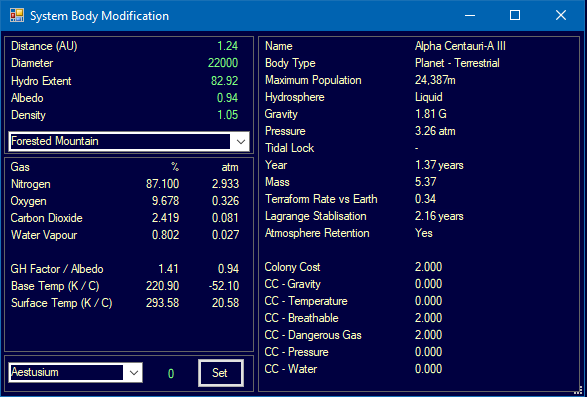
\includegraphics[width=0.5\linewidth]{images/SystemBodyModification}
		\caption[System Body Modification]{System Body Modification}
		\label{fig:systembodymodification}
	\end{figure}
	
	For example, here is what happens if the diameter is halved. Gravity, mass and max population all fall, while the terraform rate vs Earth and the time to stablise a Lagrange point both increase.
	\begin{figure}[H]
		\centering
		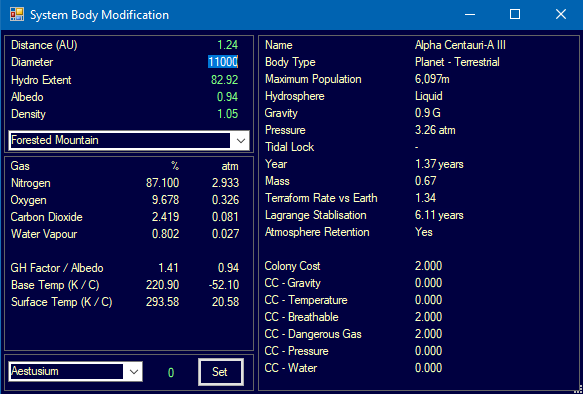
\includegraphics[width=0.5\linewidth]{images/SystemBodyModification2}
		\caption[System Body Modification 2]{System Body Modification Result}
		\label{fig:systembodymodification2}
	\end{figure}
\end{document}